% arara: lualatex: {shell: 1}
\documentclass{report}
\newif\ifprompts{}
\promptstrue{}
\input{$HOME/Dropbox/Documents/TeX/math-pre.tex}
\usepackage[nameinlink]{cleveref}
\usepackage{fancyvrb}
\usepackage{caption}
%\newcolumntype{C}{>{\begin{math}}c<{\end{math}}}
%\DeclareMathOperator{\SPN}{\text{SPN}}
\setmonofont[Scale=MatchLowercase,Contextuals={Alternate}]{FuraCode Nerd Font}
%\setminted{frame=lines,framesep=1em,fontsize=\small}
\usemintedstyle{gruvbox-light}
\setminted{autogobble,breaklines}
\hypersetup{
    colorlinks=true,
    linkcolor=BlueViolet,
    urlcolor=Bittersweet,
    citecolor=RoyalPurple,
}
\setlist{
    %itemsep=1em,
    %first={\setlength{\parskip}{1em}}
}
\setlength{\parindent}{2em}
\setlength{\parskip}{1em}
\newenvironment{code}{\captionsetup{type=listing}}{}
\newcommand{\colorA}{RoyalBlue}
\newcommand{\colorB}{PineGreen}
\newcommand{\colorC}{OrangeRed}
\addbibresource{references.bib}
\begin{document}

\title{%
    Quadratic Sieve Algorithm \\[1em]
    {\large (and trying to get it to work)}
}
\author{Nils Olsson}
\date{Spring Semester, 2021}
\maketitle

{
    \hypersetup{linkcolor=.}
    \tableofcontents
}


\pagebreak

\chapter{Abstract}

This report serves as a summary of the developmental history and mathematical theory behind
factoring functions that utilize congruences of squares, including Fermat's method, random squares
factoring, Dixon's method, and the quadratic sieve (QS) algorithm; the second half consists of a
conceptual introduction to the Rust programming language, serving more as a retrospective upon my
attempted implementation of the QS algorithm.

\section{Introduction}

The factorization of integers has been an especially well studied problem,
and not just for centuries but in fact millennia.
Greek mathematicians studied the problem, even proving the fundamental theorem
of arithmetic: that every integer has a unique prime factorization.
As a corollary the Greeks had also extensively studied the prime integers,
with the sieve of Eratosthenes being one of the most important algorithms
for generating primes ever invented.
The so called father of geometry Euclid of Alexandria (whose now self-titled
``Euclid's lemma'' was foundational for proving integer factorization
uniqueness) described in his \emph{Elements} the Euclidean algorithm for
calculating the greatest common divisor of two integers.
These ancient algorithms, and many others, comprise the fundamental building
blocks for which all modern integer factorization algorithms are made.

Number theorists to this very day strive to push factorization algorithms to their furthest,
attempting to find increasingly efficient methods of factoring large composite numbers.
With the advent of computers in the 20th century, algorithms could now leverage centuries of
man-hour's worth of computational work, and by the 80's several bleeding-edge algorithms
had been invented and tested; in particular Dixon's random squares method, the quadratic sieve (QS)
algorithm, and several others.

In this report I seek to build an understanding of not just the mathematics behind such algorithms
but the thought processes in developing such algorithms; the impetus behind them. This leads into
a broader retrospective on my own experiences in implementing these algorithms in the Rust
programming language (having effectively implemented them in Python).

\pagebreak

\chapter{Factoring via Congruences of Squares}

In this section we will cover several factorization algorithms and the fundamental math that they
are based upon. These individual topics lead-up to covering the quadratic sieve (QS) algorithm
in detail.

Something to pay special attention to is the conditions on the parameters for various algorithms,
because many of the factoring algorithms which we will discuss are \emph{not} complete factoring
algorithms. In fact, all but one is: trial division.

\section{Trial Division}
At its simplest, the task of fully finding the prime factorization of integer, and the task
determining if said integer is prime is the same task. The simplest method of doing so is what we
call \emph{trial division}.
If $n$ is the integer we wish to factor, then with trial division we consider an integer $d$ in the 
range of $2$ to the first integer greater-than or equal-to the square root of $n$ (since $\sqrt n$ is
precisely the largest number which divides $n$) with which we attempt to divide $n$.
The process is as follows:

With $d=1,2,3,\ldots$ determine if $n$ is divisible by $d$. If $n$ is divisible by $d$, we take note
of both $d$ and $e$ the power of $d$ which divides $n$, and let $n \gets n/d^e$. We only stop when
$d\not\le\ceil{\sqrt n\,}$.

With the algorithm having terminated, we know the prime power factorization of $n$ given the $d$
divisors and their corresponding $e$ exponents that we collected. If none of the $d$ divisors ever
divided $n$ then we can say with absolute certainty that $n$ is prime. This algorithm is simple
enough to implement in Python in but a few lines of code:
\begin{minted}{python}
    # Factor an integer via trial division
    # @param n Integer to factor
    # @return Its prime power factorization
    def factor_trial_division(n):
        fs = []
        d = 2
        root = ceil(sqrt(n))
        while d <= root and n > 1:
            e = 0
            while n % ] == 0:
                n //= d
                e += 1
            if e > 0:
                fs += [(d, e)]
                root = ceil(sqrt(n))
            d += 1
        if n > 1:
            fs += [(n, 1)]
        return fs

    # # Examples
    # ```
    # assert(factor_trial_division(73583) == [(73583, 1)])
    # assert(factor_trial_division(73584) == [(2, 4), (3, 2), (7, 1), (73, 1)])
    # ```
\end{minted}
Despite the naïveté of the algorithm, the trial division algorithm is often one of the very fastest
when it comes to factoring small integers. In particular, if the integer to factor is a power of
only two then trial division will outperform any of the other, more complex algorithms that we will
soon cover. In fact, the main topic of this paper---the quadratic sieve algorithm---fails entirely
not only for factoring primes but for factoring perfect powers in particular. (We will in fact be
using trial division for one of the integral steps in some of the later algorithms.)

\section{Fermat's Method}
Named after Baroque lawyer and mathematician Pierre de Fermat, Fermat's method of factorization
relies on a simple fact: that any odd integer is equal to the difference of squares.

\newcommand{\bdot}{
\begin{tikzpicture} \fill[\colorA] (0,0) circle(3pt); \end{tikzpicture}}
\newcommand{\pdot}{
\begin{tikzpicture} \fill[\colorB] (0,0) circle(3pt); \end{tikzpicture}}
\newcommand{\rdot}{
\begin{tikzpicture} \fill[\colorC] (0,0) circle(3pt); \end{tikzpicture}}
\columnratio{0.6}
\begin{paracol}{2}
    \noindent
    As a simple visual proof of this fact, let $N$ be any odd integer
    \cite{illustrated}.
    By definition of $N$ being odd, $N=2m+1$ for some integer $b$.
    \begin{enumerate}
        \item Draw a single \pdot{} dot capped on either side by $m$ \bdot{} dots.
            The count of these dots is clearly $N$.
        \item Bend the right side of \bdot{} dots down to form a square.
        \item Fill the square with more \rdot{} dots.
    \end{enumerate}
    Then clearly the area of the whole square minus the area of the inner square
    of only \rdot{} dots is equal to $N$ (a difference of squares).

    \switchcolumn

    \begin{enumerate}[itemsep=3em]
        \item
            \adjustbox{center,valign=t,raise=-2pt}{%
                
\begin{tikzpicture}
                    \foreach \i in {0,...,2} { \fill [\colorA] (0.5*\i,      0) circle(3pt); }
                    \fill [\colorB] (1.5,0) circle(3pt);
                    \foreach \i in {4,...,6} { \fill [\colorA] (0.5*\i,      0) circle(3pt); }
                \end{tikzpicture}
            }
        \item
            \adjustbox{center,valign=t,raise=-2pt}{%
                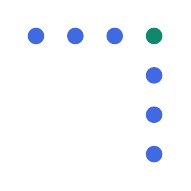
\begin{tikzpicture}
                    \foreach \i in {0,...,2} { \fill [\colorA] (0.5*\i,      0) circle(3pt); }
                    \fill [\colorB] (1.5,0) circle(3pt);
                    \foreach \i in {1,...,3} { \fill [\colorA] (   1.5, -0.5*\i) circle(3pt); }
                \end{tikzpicture}
            }
        \item
            \adjustbox{center,valign=t,raise=-2pt}{%
                
\begin{tikzpicture}
                    \foreach \i in {0,...,2} { \fill [\colorA] (0.5*\i,      0) circle(3pt); }
                    \fill [\colorB] (1.5,0) circle(3pt);
                    \foreach \i in {1,...,3} { \fill [\colorA] (   1.5, -0.5*\i) circle(3pt); }
                    \foreach \x in {0,...,2} {
                        \foreach \y in {1,...,3} {
                            \fill [\colorC] (0.5*\x, -0.5*\y) circle(3pt);
                        }
                    }
                \end{tikzpicture}
            }
    \end{enumerate}
\end{paracol}
And if neither $a+b$ nor $a-b$ equal one or $N$, then they are \emph{non-trivial} factors of
$N$ (the trivial factors of $N$ being $1$ and $N$ itself).

With this fact in hand, let $n$ be an odd composite integer; we wish to find $c$ and $d$ such that
$n=cd$.
(Note that we are only interested in odds since, if $n$ were even, we simply factor out all copies
to $2$ until all that is left is supposedly an odd composite.) We know that for some $a$ and $b$
with $n=a^2-b^2$ that the difference of squares is factorable into $(a+b)(a-b)$. This implies
$c=a+b$ and $d=a-b$ with which we derive $a=(c+d)/2$ and $b=(c-d)/2$. We can verify:
\[
    n
    = {\left(\frac{c+d}{2}\right)}^2-{\left(\frac{c-d}{2}\right)}^2
    = \frac{(c^2+2cd-d^2)-(c^2-2cd+d^2)}{4} = cd.
\]
Rewriting the difference of squares statement as $b^2=a^2-n$,
and without loss of generality letting $a\ge\sqrt{n}>b$,
the goal of Fermat's method in one way or another is to attempt to find an $a$
satisfying the \emph{strict} relationship $b=\sqrt{a^2-n}$ where $b$ is an integer.
We can similarly implement this algorithm easily in Python but just checking all integers
from $\ceil{\sqrt{n}\,}$ to $n$.
Square roots are relatively cheap, but we do require a method of checking whether a root is an
integer (we use $[b^2]\overset{?}{=}{\ceil b}^2$):
\begin{minted}{python}
    # Find two factors of an odd integer via Fermat's method
    # @param n Odd integer to factor
    # @return Two factors (possibly trivial)
    def factor_fermat(n):
        for a in range(ceil(sqrt(n)), n + 1):
            b = sqrt(a**2 - n)
            if int(b**2) == ceil(b)**2:
                return(int(a + b), int(a - b))

    # # Examples
    # ```
    # assert(factor_fermat(811) == (811, 1))
    # assert(factor_fermat(813) == (271, 3))
    # ```
\end{minted}
As such there's not much improvement in terms of the complexity of this algorithm when compared to
trial division; at worst case we have checked $\ceil{\sqrt{n}\,}$ integers when $n$ is prime.
Further more, we can only use this algorithm when $n$ is odd, and we only get two particular factors
for $n$. However, it is incredibly simple in this regard, and of course this simple implementation
would only be part of a complete factoring algorithm which we could achieve by factoring 2 out from
any even $n$ to to form an odd $n$, factoring every odd $n$ via Fermat's method, and factoring each
non-trivial resultant factor for as long as it takes until having completely factored $n$.

\section{Congruences of Squares}

In contrast, consider this \emph{less-strict} congruence relation:
\[
    a^2 \equiv b^2 \pmod n
    \Rightarrow
    a^2-b^2 = (a+b)(a-b) \equiv 0 \pmod n.
\]
If $n$ divides $(a+b)(a-b)$, then $\gcd(a+b,n)$ and $\gcd(a-b,n)$ certainly both yield factors of
$n$. However, if $a\pm b\equiv 0\pmod n$, then $\gcd(a\pm b,n)=n$ or 1, the trivial factors of $n$.
So in addition to $a^2\equiv b^2\pmod n$ we add the constraint that $a\not\equiv\pm b\pmod n$, such
that neither $a+b$ or $a-b$ are divisible by $n$. And \emph{if we find} a pair $a$ and $b$
satisfying these two less-strict congruence relations
\begin{gather}
    a^2 \equiv b^2 \pmod n, \label{eq:square-congruence1} \\
    a \not\equiv \pm b \pmod n \label{eq:square-congruence2}
\end{gather}
We have non-trivial factors of $n$.

Further more, the condition $a^2\equiv b^2\pmod n$ is that of $b^2$ being a \emph{quadratic residue}
modulo $n$. We say an integer $y$ is a quadratic residue modulo $n$ if there exists an $x$ such that
$x^2\equiv y\pmod n$, and if no such $x$ exists we call $y$ a quadratic non-residue.
If instead we take a prime $p$ to be our modulus, then we have as a fact
that of the integers from $0$ to $p-1$ half are quadratic residues modulo $p$ when $p$ is odd
(on the other hand, every integer is a quadratic residue modulo $2$).
Explicitly, we have the \emph{Legendre symbol} of $a$ modulo odd prime $p$:
\begin{equation}
    \left(\frac{a}{p}\right)
    = a^{p-1/2}\pmod p
    \equiv \begin{cases}
        \phantom{-}0, & \text{if $p$ divides $a$,} \\
        \phantom{-}1, & \text{if $a$ is a quadratic residue modulo $p$, or} \\
        -1, & \text{if $a$ is a quadratic non-residue modulo $p$.}
    \end{cases}
\end{equation}
(These equivalent forms were expressed historically by Legendre and Euler.)
The \emph{Jacobi symbol} $\left(\frac{a}{n}\right)$ generalizes the Legendre symbol for
when instead the modulus is a composite $n$
\cite{textbook}.
Both the Legendre and Jacobi symbols have many
useful properties, but in particular if $n$ has the prime factorization
$p_1^{e_1}p_2^{e_2}\cdots p_k^{e_k}$, then we have that the Jacobi symbol of $a$ modulo $n$
can be expressed as the product of powers of the Legendre symbols over each prime:
\begin{equation}
    \left(\frac{a}{n}\right) =
    {\left(\frac{a}{p_1}\right)}^{e_1}
    {\left(\frac{a}{p_2}\right)}^{e_2}
    \cdots
    {\left(\frac{a}{p_k}\right)}^{e_k}.
\end{equation}

Returning to the problem of factoring $n$, the question remains:
\emph{how do we find $a$ and $b$ pairs satisfying \cref{eq:square-congruence1} and
\cref{eq:square-congruence2}?}
The most naïve method would be to pick pairs $a$ and $b$ at random, hoping for a collision
satisfying the conditions (but we will not exactly consider this an algorithm).

\section{Dixon's Random Squares Algorithm}

Consider that a composite integer is a perfect square only if every prime in its prime factorization
is raised to a positive power (that is, every exponent has even parity). Factoring algorithms of the
\emph{random square} variety seek to find find ``small'' composite integers such that their product
yields a perfect square in this sense, to then solve the problem of congruences of squares.
Dixon's algorithm/random squares method is one of such algorithms.

To do so practically, instead of factoring over the set of all the primes we select a subset $\cB$
of the $t$ first primes. We call this our \emph{factor base}, $\cB = \{p_1,p_2,\ldots,p_t\}$.
We say that an integer $n$ is \emph{$p_t$-smooth} if the largest prime factor of $n$ is less-than or
equal-to the $t^\text{th}$ prime, and thus smooth over our factor base of all the primes up to $p_t$.

And instead of looking for $a$ and $b$ pairs satisfying the (already weak) conditions from previously,
by Dixon's method we look for integers $a_i$'s which satisfy the \emph{even weaker still} relation
$a_i^2\equiv b_i\pmod n$ and where the $b_i$ we calculate is smooth over our factor base
(this step of checking whether $b_i$ is $p_t$-smooth requires at least trial division and thus
determining its prime factorization---we will need this later).
In Dixon's method, the selection of these various $a_i$'s can be random, but considering that trial
division may be expensive it is favorable to find them in a way where $b_i\pmod n$ ends up small.
Two such ways, with integers $j\ge 0$ and $k\ge 1$, are $j+\ceil{\sqrt{kn}}$ and
$\floor{\sqrt{kn}}$; the former produces integers $a_i^2\pmod n$ that tend small, and
the later produces integers $-a_i^2\pmod n$ that also tend to be small \cite{handbook}.
(One thing to note is that in the case of the later we need to add $p_0=-1$ to the
factor base to be able to factor anything negative; ultimately this doesn't change
anything about the algorithm aside that it can greatly improve the speed at which we find pairs
since we have twice as many potential small $a_i$'s.)

But once we have found pairs $(a_i,b_i)$ satisfying $a_i^2\equiv b_i\pmod n$ and $b_i$ is
$p_t$-smooth, \emph{what do we do with them?} Recall the consideration (three paragraphs back) that
an integer is a perfect square if and only if its prime power factorization is of even powers of
primes. For each of the $(a_i,b_i)$ pairs we express $b_i$ as a product of powers of the primes in
$\cB$ our factor base and record these exponents as vectors in both decimal and over the field
$\ZZ_2$:
\begin{equation}
    b_i = p_1^{e_{i1}}\cdot p_2^{e_{i2}}\cdots p_t^{e_{it}}
    \quad\Rightarrow\quad
    \vec e_i = \langle e_{i1},e_{i2},\ldots,e_{it}\rangle
    \quad\Rightarrow\quad
    \vec v_i = \langle v_{i1},v_{i2},\ldots,v_{it} \rangle
\end{equation}
For each $p_j\in\cB$, and where $v_{ij}\equiv e_{ij}\pmod 2$ (i.e.\@ the parity of $e_{ij}$).
Recall that we know the prime power factorization of $b_i$ from checking that $b_i$ is $p_t$-smooth
via trial division. If the sum of a subset of these $\vec v_i$ equals the zero vector, \emph{then we
have found a congruence of squares satisfying $a^2\equiv b^2\pmod n$}, just with a few extra steps
left to construct $a$ from the $a_i$'s and $b$ from the $b_i$'s. In terms of linear algebra, we have
found a linearly dependent subset of the $\vec v_i$ vectors. This clues us into quantifying how many
$(a_i,b_i)$ pairs we need to \emph{guarantee} that we actually have enough such pairs:

\noindent
Our vectors have $t$ columns, one for every prime in $\cB$ the factor base; if we form a matrix of
the vectors, then the rank of this matrix is at most $\abs{\cB}$ the number of columns; lastly, if
the number of rows of the matrix is equal to one plus its rank (the number of columns), then we
\emph{guarantee} that the row space contains linear dependencies (since fundamentally the row rank
and column rank of a matrix are always equal, and at ``worst'' the column space is entirely linearly
dependent with rank $\abs{\cB}$).

\noindent
Thus we need \emph{at least} $\abs{\cB}+1$ $(a_i,b_i)$ pairs to guarantee that we can construct a
congruence of squares.

Constructing $a$ and $b$ is actually fairly straight forward:
let $I\subseteq\{1,2,3\ldots,t\}$ be the set of indices $i$ for which we found
$\sum_{i\in I}\vec v_i = \vec 0$.
Fix $b^2$ to be:
\begin{equation}\label{eq:dixon-forming-a2-b2}
    b^2 = \prod_{i\in I} b_i = \prod_{j=1}^t p_j^{\epsilon_j}
    \equiv \Big(\prod_{i\in I}a_i\Big)^2 = a^2 \pmod n.
\end{equation}
Where each $\epsilon_j = \prod_{i\in I} e_{ij}\equiv 0\pmod 2$ has positive parity,
and therefore we know $b^2$ to be a perfect square.
Thus we can construct $b$ by simply dividing each $\epsilon_j$ by two:
\begin{equation}
    b = {\Big(\prod_{i\in I} b_i\Big)}^{1/2} = \prod_{j=1}^t p_j^{\epsilon_j/2}.
\end{equation}
It suffices to calculate $a=\prod_{i\in I}a_i$ since we already have that $a^2$ is clearly a perfect
square in the satisfied congruence relation \cref{eq:dixon-forming-a2-b2}.

Despite all the work we have done, if we find that $a\equiv \pm b\pmod n$ then the pair $(a,b)$
has unfortunately failed to yield anything but the trivial factors of $n$.
As for our avenues of recourse, we can:
\begin{enumerate}
    \item Check for other linearly dependent subsets $I$ and their corresponding pairs $(a,b)$. If
        every subset failed, then
    \item We can search for more $(a_i,b_i)$ pairs (we call this increasing the search interval),
        perform the previous actions all over again but with these new pairs, then if that fails
    \item Start over with an expanded factor base.
\end{enumerate}

One question we have ignored is \emph{how do we select a satisfactory factor base?}
The scope of this question is beyond my intent for this paper, but the optimal selection for $t$,
based upon the study of smooth integers near arbitrary $\sqrt n$, is supposedly near to $L_n[\frac 1
2,\frac 1 2]$, where
\[
    L_q[\alpha,c]
    = O(\exp((x+o(1))(\ln q)^\alpha(\ln \ln q)^{1-\alpha}))
\]
But frankly this is beyond my knowledge of complexity.
\cite{handbook}.

A second question could concern the sieving interval.
Clearly we have a minimum number of $(a_i,b_i)$ pairs for linear dependence, but by my judgmet
we might as well find more than we ``need'', should several linear dependent cases fail to produce
any pair such that $a_i\not\equiv b_i1\pmod n$.

\section{The Quadratic Sieve Algorithm}

Last but not least we discuss the QS algorithm, but despite all this lead-up there is truly not that
much more to it in comparison to Dixon's. The QS algorithm functions almost identically to Dixon's
method, except for the way in which potential $a_i$'s are selected: first by a simple translation,
and second in actual ``sieving.''

Letting $n$ be the integer to factor and $m=\floor{\sqrt n}$, consider the polynomial:
\begin{equation}
    f(x)=(x+m)^2-n.
\end{equation}
In Dixon's algorithm we selected $a_i$'s either randomly or using a slight
heuristic. Instead, in the QS algorithm we select $a_i=(x+m)$, calculate a corresponding
$b_i=f(x)=(x+m)^2-n$ and test whether $b_i$ is $p_t$-smooth (just like in Dixon's).
Note the relationship between $a_i$ and $b_i$ pair:
\begin{equation}
    a_i^2
    = (x+m)^2
    = (x+m)^2 - n + n
    \equiv (x+m)^2 - n
    = b_i \pmod n.
\end{equation}
Identical to the congruence relation from Dixon's.
Recall that we want the $b_i$'s to factor entirely over our chosen factor base $\cB$ (that is to be
$p_t$-smooth), but suppose $b_i$ is divisible by some prime $p$ in general. Then $p$ also divides
$(x+m)^2-n$ (from our definition of $b_i$), which gives us
\begin{equation}
    (x+m)^2 - n \equiv 0 \pmod p \Rightarrow
    (x+m)^2 \equiv n \pmod p.
\end{equation}
Clearly $(x+m)^2$ is a square, meaning that $n$ is a quadratic residue (modulo $p$)!
Therefore we can narrow down the factor base to contain only those primes $p_j$ such that
$n$ the integer we wish to factor is itself a quadratic residue modulo $p$.
And from here we have all the tools we need to begin search for $(a_i,b_i)$ pairs in a fashion
practically identical to that in Dixon's. The sequence $x=0,\pm 1,\pm 2,\ldots$ keeps each
corresponding $b_i$ fairly small in absolute value (similar to the heuristics in Dixon's).

However, \emph{what of the sieving?}
Up to now, validating each $b_i$ has consisted of trial division.
This method is easy and not terrible for numbers that are not too big but the performace cost it
imposes upon the data collection stage of the algorithm (the collecting of the pairs) is high.
Lets consider the following family of functions $f(x+kp)$ where $p$ is an odd prime and $k$ an
integer:
\begin{equation}
    \begin{aligned}
        f(x)=(x+m)^2-n \Rightarrow
        f(x+kp)
        &= ((x+kp)+m)^2 - n \\
        &= x^2+2xkp+2xm+(kp)^2+2kpm+m^2-n \\
        &= (x^2+2xm+m^2-n) + (2xkp+(kp)^2+2kpm) \\
        &= ((x+m)^2-n)+p(2xk+k^2 p+2km) \\
        &\equiv f(x) \equiv (x+m)^2 \pmod{p}.
    \end{aligned}
\end{equation}
Thus if we can solve $f(x) = (x+m)^2 \equiv 0\pmod p$ for $x$ then for every root $r$ we find we
have an \emph{entire sequences} of numbers $\{f(x):x=0,\pm 1,\pm 2,\ldots,\pm I\text { and }x\equiv
r\pmod p\}$ (for sieving interval $I$) for which \emph{every} element is in-fact divisible by the
prime $p$.
Solving for the quadratic roots here is over modulo $p$ which in itself adds another layer of
complexity; one popular algorithm for calculating these roots, which I implemented, is the
Tonelli-Shanks algorithm.
\begin{minted}{python}
    # Get two quadratic roots (or double root)
    # of an integer modulo a prime, if they exists.
    # (Tonelli-Shanks algorithm)
    #
    # @param n Integer whose roots to return
    # @param p Prime modulus
    # @return (r1,r2) Two quadratic root of n modulo p, or (None, None)
    def sqrt_mod(n, p):
        if p == 2:
            # Any integer has a double root 0 or 1 modulo 2
            r = n % 2
            return (r, r)
        if not is_quadratic_residue(n, p):
            return (None, None)
        # express p - 1 as q*2^s (where q is odd)
        q, s = div_while(p - 1, 2)
        if s == 1:
            r = pow(n, (p+1)//4, p)
            return (r, p - r)
        # find a quadratic-non residue modulo p (in this case the first)
        z = next(filter(lambda z: not is_quadratic_residue(z, p), range(2, p)))
        m = s
        c = pow(z, q, p)
        t = pow(n, q, p)
        r = pow(n, (q+1)//2, p)
        while (t - 1) % p != 0:
            # find least 0 < i < m st. t^(2^i) ≡ 1 (mod p)
            i = next(i+1 for (i, t2) in enumerate(squarings(t, p)) if (t2 - 1)
            b = pow(c, 1 << (m - i - 1), p) # b = c^(2^(m-i-1))
            r = (r * b) % p
            c = (b * b) % p
            t = (t * c) % p
            m = i
        return (r, p - r)
\end{minted}

There are several methods of initializing the values of the sieve, but in all cases the values are
indexed by the parameter $x$. In my implementation, the $x^\text{th}$ value is initialized
to $f(x)$. Then for each prime in the factor base we solve for the roots $r_1$ and $r_2$ of $f(x)$
modulo $p$ (with the possibility that $r_1=r_2$).
If the root $r_j$ exists, then every element of the sieve with index congruent to $r_j$ modulo $p$ is
divisible by $p$, and for those values we divide by $p$ (until we no longer can).
\begin{minted}{python}
    # Find p_b smooth square numbers within a sieving interval
    #
    # @param n Integer to find two non-trivial factors of
    #   (but also the quadratic polynomial linear term)
    # @param b Desired factor base length
    # @param I Sieving interval
    # @return List of sieved x's, of y's (corresponding in parallel with the x's
    #   as smooth pairs), and the factor base
    def find_smooth(n, b, I):
        m = ceil(sqrt(n))
        # Sieve from sieving interval
        V = [(x + m)**2 - n for x in range(I)]
        # In tandem, find b primes p for which n has roots modulo p
        p_root_pairs = list(take(b, iter_roots(n)))
        fb, roots = zip(*p_root_pairs)
        # Sieve!
        for (p, roots) in p_root_pairs:
            for r in roots:
                start = (r - m) % p
                for i in range(start, len(V), p):
                    while V[i] % p == 0:
                        V[i] //= p
        # Construct, collect and return the x's and y's (which are smooth)
        xs = [i + m for (i, v) in enumerate(V) if abs(v) == 1]
        ys = [x**2 - n for x in xs]
        return (xs, ys, fb)
\end{minted}
Once we have done this for every $p$ in the factor base, we know that whenever we see a value of 1
within the sieve that the initial value was not just $p_t$-smooth \emph{but also entirely
factorable} over the factor base. We can recalculate from the indices $x$ the initial values for
$b_i$ that we now know are factorable as we desire (and as far as prime factorization goes, we can
divide by primes only in the factor base and still receive a full prime power factorization).
And from here we find ourselves back at Dixon's method, solving for linear dependencies within
the points we sieved for, which concludes the main object of this first-half.

\emph{
    But as a reminder, the quadratic sieve algorithm, like Dixon's method, and like random squares,
    serves a specific purpose with a larger factoring algorithm. QS is absolutely not going to be the
    fastest algorithm for a very large amount of potential inputs, and often we shouldn't use
    QS until having at least tried both trial division and Fermat's methods for several values.
}

The following is some test runs of my implementation of the algorithm, timed using the
\mintinline{bash}{time} command execution utility. The results were cherry picked to at least
be composites.
It is no where near as efficient as I can make it, but this Python version was more for learning
and verifying how the algorithm works, in rough detail.
After the sample output is a snippet of the code of my implementation, specifically the highest
scope of the algorithm, \mintinline{python}{def qs(n, b, I)}, and parts of the matrix operation
functions I also needed to implement to be able to find the linear dependencies efficiently.
(The first iteration of my implementation simply tried all combinations, but this rather quickly
and obviously got out of hand for large factor bases.)

All that is left is to discuss the programming itself, and some of the particular challenges I faced
during the implementation of the QS algorithm.
\begin{minted}{bash}
    > time python3 qs-sieving.py 16843009979 50 4000
    (881, 19118059)
    python3 qs-sieving.py 16843009979 50 4000  0.34s user 0.10s system 115% cpu 0.375 total

    > time python3 qs-sieving.py 16843812359755 300 15000
    (31667, 531904265)
    python3 qs-sieving.py 16843812359755 300 15000  1.23s user 0.09s system 127% cpu 1.032 total

    # the following are products of two primes

    # notice that we could have used trial division here
    # and found non-trivial factors within 4 iterations, when d=5,
    # much much faster than QS
    > time python3 qs-sieving.py 16843812359755 250 15000
    (3368762471951, 5)
    python3 qs-sieving.py 16843812359755 250 15000  1.01s user 0.10s system 136% cpu 0.807 total

    # but for this result, trial division would have failed miserably in needing to check up to
    # 73477 (since both these factors are prime). Fermat's would need to check approximately
    # 98669-sqrt(7249902113) = 13523 values
    > time python3 qs-sieving.py 7249902113 50 4000
    (98669, 73477)
    python3 qs-sieving.py 7249902113 50 4000  0.27s user 0.06s system 162% cpu 0.206 total

    > time python3 qs-sieving.py 30240256903 50 4000
    (45631, 662713)
    python3 qs-sieving.py 30240256903 50 4000  0.31s user 0.09s system 64% cpu 0.617 total
\end{minted}
\pagebreak
\subsubsection*{Excerpts of the Python implementation}
\begin{minted}{python}
    # Quadratic sieve
    #
    # My implementation of a single-polynomial quadratic sieve.
    #
    # @param n Integer to find two non-trivial factors of
    # @param b Desired factor base length
    # @param I Sieving interval
    def qs(n, b, I):
        xs, ys, fb = find_smooth(n, b, I)
        # ...
        for indices in combinations(range(len(xs)), len(fb)+1):
            xs_ = [xs[i] for i in indices]
            ys_ = [ys[i] for i in indices]
            emat, bmat = construct_exponent_mats(ys_, fb)
            # The augmented binary matrix is for solving for the left nullspace,
            # and thus all the subsets of linearly dependent exponent vector indices.
            for indices in ld_index_iter(bmat):
                x = prod(xs_[i] for i in indices)
                l = [sum(emat[i][j] for i in indices) // 2 for j in range(len(fb))]
                y = prod(p**e for (p, e) in zip(fb, l))
                if not x % n in [y % n, -y % n]:
                    return (gcd(x + y, n), gcd(x - y, n))

    # Iterator over linearly dependent row index subsets of a binary matrix.
    # (Refer to the notes in the to_echelon_form function about how to find
    # linearly dependent row index subsets.)
    #
    # @param mat Matrix
    # @yields Subset of binary matrix row indices in left-nullspace
    def ld_index_iter(bmat):
        n = len(bmat[0])
        bmat_aug = augment(bmat)
        bmat_echelon = to_echelon_form(bmat_aug)
        for i in range(len(bmat_echelon)):
            if all(a == 0 for a in bmat_echelon[i][:n]):
                coords = bmat_echelon[i][n:]
                indices = [i for (i, b) in enumerate(coords) if b]
                if len(indices) > 0:
                    yield indices

    # Bring binary matrix into echelon form.
    #
    # If the matrix to bring to echelon form is an augmented matrix, then in
    # echelon form the sub-rows within the augmentation sub-matrix correspond to
    # subsets of the row indices of the original matrix that are linearly dependent
    # modulo 2 (i.e. in the left nullspace).
    #
    # @param mat Matrix to operate over
    # @return Computed echelon form matrix
    def to_echelon_form(mat):
        mat = deepcopy(mat)
        #...
\end{minted}

\subsection{Additional Notes on QS}

The QS algorithm as we have discussed is only one particular conceptualization of the algorithm.
One variation considers that if we have integers $a_1^2$ and $a_2^2$ that are \emph{not} $p_t$-smooth
(smooth over our chosen factor base), there may may be a way to combine their partial relations
to form a third composite of $a_1$ and $a_2$ that \emph{is} $p_t$-smooth. For example (as
\href{https://en.wikipedia.org/wiki/Quadratic_sieve#Partial_relations_and_cycles}{sourced from Wikipedia})
if $n=91$ and $\cB=\{2,3,5,7\}$, integers $a_1^2={21}^2\equiv 7\cdot 11\pmod{91}$ and
$a_2^2={29}^2\equiv 2\cdot 11\pmod{91}$ are not 7-smooth. However, if we multiply these together
\begin{align*}
    (21\cdot 29)^2
    &\equiv 2\cdot 7\cdot 11^2 \pmod{91} \\
    ({11}^{-1})^2\cdot (21\cdot 29)^2
    \equiv (58\cdot 21\cdot 29)^2
    &\equiv 2\cdot 7 \pmod{91}.
\end{align*}
We find a $p_t$-smooth integer.

Secondly, we only considered the QS algorithm for a single polynomial $f(x)=(x+m)^2-n$,
where we could if careful select multiple polynomials of a particular family.
The advantage to this variation is the potential to sieve within each polynomial in parallel
across multiple CPU threads.

Lastly, inventor of the QS algorithm Carl Pomerance conjectures \cite{pomerance}
that it has complexity of order
\[
    O(\exp((1+o(1))(\log n\log\log n)^{1/2}).
\]
This places it within the category of sub-exponential functions,
similar to the one algorithm that is faster than QS---the general number field sieve (GNFS)---which
has the following conjectured complexity \cite{wiki-gnfs}:
\[
    O\left((\exp\left({\left(\frac{64}{9}\right)}^{1/3}+o(1)\right)(\ln n)^{1/3}(\ln\ln n)^{2/3}\right).
\]
And as such QS is slightly worse in comparison to GNFS, thought they both lie
within the category of sub-exponential functions.

\chapter{Notes on Implementation}

I decided to designate the implementation discussion to the Rust implementation alone.
Not because it is more complete than
the Python implementation (on the contrary even), but because I find it vastly
more interesting, and because I included much of the Python implementation in the previous half
of this report. Still, the Python implementation works; I wrote it primarily as a sanity
check (it is definitely easier and faster to bang-out an implementation in
Python than Rust) and its entirety can be found here:\\
\href{https://github.com/nilsso/quadratic-sieve-rs/tree/main/python-version}{github.com/nilsso/quadratic-sieve-rs/python-version/}.

For those who wish to peruse it, begin in the
\href{https://github.com/nilsso/quadratic-sieve-rs/blob/main/python-version/qs-sieving.py}{qs-sieving.py}
module, which can then lead you to the other modules and how they are used
(like the Tonelli-Shanks
\href{https://github.com/nilsso/quadratic-sieve-rs/blob/main/python-version/sqrt\_mod.py#L22}{sqrt\_mod}
algorithm, which leads to the Legendre symbol implementation, the \mintinline{rust}{is_quadratic_prime}
function and the \mintinline{rust}{legendre_primes} iterator in
\href{https://github.com/nilsso/quadratic-sieve-rs/blob/main/python-version/legendre.py}{legendre.py}).

With the fundamental algorithm completed in Python, I made my move to Rust.
This section is primarily a retrospective on my experience in implementing \emph{(or at
least attempting to implement)} the QS algorithm in Rust. I intend for it to be useful to anyone
with an interest in Rust, as well as useful to myself in both reviewing my own knowledge of the
language and providing a figurative map of my thoughts on the design of my project's implementation.
I go over the Rust language in general, how its features have been very useful for implementing
mathematical structures, and weave in how I used these features in my own QS implementation. If
heavy use of programming jargon is not your thing then this section may not be very interesting.
That being said, the full source code of the Rust portion of this project can be found here:
\href{https://github.com/nilsso/quadratic-sieve-rs/tree/main/src}{github.com/nilsso/quadratic-sieve-rs/}.

\section{Implementing in Rust}

As far as fundamental paradigms go, Rust as a programming language has much in
common with more classically object oriented languages like C++ or Java, but
also a lot in common with purely function languages like Haskell.
Similarities with the later are in Rust's sophisticated \emph{trait} feature,
analogous to Haskell's \emph{type classes}, with which Rust acomplishes
polymorphism.
In C++, polymorphism in achieved through hierarchies of \mintinline{cpp}{class}es and
abstract \mintinline{cpp}{classes} (i.e. interfaces)
(e.g.\@ if a \mintinline{rust}{Square} derives from \mintinline{rust}{Shape}, then a function which
accepts a \mintinline{rust}{Shape} can accept a \mintinline{rust}{Square}).
Although Rust encapsulates data and functionality through \mintinline{rust}{struct}s
(analogous to C++ \mintinline{cpp}{class}es) and their instantiations,
polymorphism in Rust is achieved \emph{only} through its traits
(e.g.\@ if \mintinline{rust}{Shape} is a trait and \mintinline{rust}{Square} implements the \mintinline{rust}{Square}
trait, then a function that requires its argument implement \mintinline{rust}{Shape} can
accept a \mintinline{rust}{Square}).

The most substantial difference in polymorphism is that there is \emph{no such
thing} as inheritance for Rust \mintinline{rust}{struct}s like there is for C++
\mintinline{cpp}{class}es. (e.g. in C++, \mintinline{rust}{Square} as a \mintinline{cpp}{class} is a subclass of
an abstract class \mintinline{rust}{Shape};
in Rust, \mintinline{rust}{Square} \emph{implements} \mintinline{rust}{Shape}, where \mintinline{rust}{Square} is a
\mintinline{rust}{struct} and \mintinline{rust}{Shape} is a \mintinline{rust}{trait}. Further more, \emph{if
\mintinline{rust}{Shape} was a \mintinline{rust}{struct} instead of a \mintinline{rust}{trait}},
\mintinline{rust}{Square} could not inherent any of \mintinline{rust}{Shape}'s functionality and neither
would share any functionality---as far as the compiler is concerned---without
them both implementing some other trait.)
This is a major paradigm shift for anyone moving from C++ to Rust, as
inheritance based polymorphism is more-or-less the only flavor of polymorphism
that students of computer science/programming are likely to have learned (as was
the case for me especially), and one might believe on a first glance that if
inheritance is not a feature then Rust \mintinline{rust}{struct}s cannot share functionality
without copying entire swathes of code.

Instead, Rust \mintinline{rust}{trait}s fill this purpose: a \mintinline{rust}{trait} can define default
functionality for which any \mintinline{rust}{struct} which implements the trait inherits.
For example, the code in \cref{fig:trait-demo} defines a trait \mintinline{rust}{Pow}
representing the capability of the implementing type to be ``raised to a
power,'' for which any type can implement. (A note on the language: an
\mintinline{rust}{impl} block \emph{implements} functionality, i.e.\@ one or several
functions, onto an existing type. These can be \emph{methods} for instances of
the type, like \mintinline{rust}{a.foo()}, or \emph{functions} belonging to the type itself,
like \mintinline{rust}{Foo::foo()}.)
\begin{code}
    \begin{minted}{rust}
        trait Pow {
            /// Raise this value to an exponent.
            /// (Must be implemented)
            fn pow(&self, e: u32) -> Self;

            /// Square this value.
            /// (Implemented by default, and does *not* need to be re-implemented)
            fn squared(&self) -> Self {
                self.pow(2)
            }
        }

        // Although we don't implement the `squared` method for `i32` here,
        // it gets the default implementation from the `Pow` trait.
        impl Pow for i32 {
            fn pow(&self, e: u32) -> i32 {
                <i32>::pow(e)
            }
            // fn squared... is inherited.
        }
    \end{minted}
    \caption{A trait with a default implementation.}
    \label{fig:trait-demo}
\end{code}
\noindent
The fundamental advantage of traits used in this way is that if we then write a
function in which we need the functionality of \mintinline{rust}{pow}, then we can require
that whatever type(s) the function works over, and/or takes as parameters,
\emph{implement the \mintinline{rust}{Pow} trait}; furthermore, anyone is allowed to
implement \mintinline{rust}{Pow} trait, and thus use our function with their own \mintinline{rust}{Pow}
implementing type. In other words, \emph{polymorphism in Rust is achieved by
abstracting over the functionality that types have, and not the types
themselves in particular}. We call these functionality requirements on types
\emph{trait bounds}.

Another advantage of trait bounds is that they allow us to add functionality to
a type \emph{incrementally} by requiring increasingly stricter trait bounds for
more functionality dependent operations. I bring up an example that I will use
continuously from now on: my implementation of $M\times N$ matrices,
\verb+Matrix+.
At its most generic, a matrix can be just a two-dimensional storage location
in which we could potentially store anything. As such, in
\cref{fig:rust-matrix-def} I define \mintinline{rust}{Matrix} without any bounds on what
it is allowed to store aside from the type needing to be clonable.
(Heed not the syntax \mintinline{rust}{const M} and \mintinline{rust}{const N}, but know that they
control the size of the matrix; we will cover this syntax in a few paragraphs
from here)
\begin{code}
    \begin{minted}{rust}
        #[derive(Clone)]
        pub struct Matrix<T, const M: usize, const N: usize>
        where
            T: Clone,
        {
            pub rows: [[T; N]; M], // M arrays of T arrays of length N
        }
    \end{minted}
    \caption{The verbatim definition of my own matrix type.}
    \label{fig:rust-matrix-def}
\end{code}
\noindent
In this snippet, \mintinline{rust}{T} is called a generic parameter, and it is given the
trait bound \mintinline{rust}{Clone}; thus we are allowed to make a matrix of type \mintinline{rust}{T}
for any type \mintinline{rust}{T} that is clonable. Personally, I find something inherently
mathematical about the way in which we can restrict generic types in Rust. This
leads me to a particular implementation (\cref{fig:rust-matrix-zero}) for my
\mintinline{rust}{Matrix} \mintinline{rust}{struct}: the zero matrix.
\begin{code}
    \begin{minted}{rust}
        impl<T, const M: usize, const N: usize> Matrix<T, M, N>
        where
            T: Zero<Element = T> + Clone,
        {
            pub fn zeroes() -> Self {
                // T::ZERO is the constant value that represents
                // zero for the generic type parameter T.
                let rows = array_init(|_| array_init(|_| T::ZERO));
                Self::from_array(rows)
            }
        }
    \end{minted}
    \caption{Implementation to construct a $M\times N$ all-zero matrix.}
    \label{fig:rust-matrix-zero}
\end{code}
\noindent
In this snippet we define the construction of a zero matrix of specified size
$M\times N$. This begs the question: \emph{how do we know
that the type \mintinline{rust}{T}, for which the matrix is over, has a representation of zero at
all?} For the generic type \mintinline{rust}{T}, the only way then for the compiler to know
that \mintinline{rust}{T} has zero is to impose an additional trait bound, in this case a
trait of my own called \mintinline{rust}{Zero}. The only thing that this trait requires is
that an implementing type provide a constant representation of zero, and with
this we have a value with which to fill a zero matrix. Additionally, note the
\mintinline{rust}{Element = T} part of the trait bound: this requires that not only
does \mintinline{rust}{T} need to have a zero element, but that the zero element \emph{must
be of the same type as \mintinline{rust}{T} itself}. This allows for a distinction when, for
example, something like a set of numbers has a zero element, but the zero
element is not itself a set (think of the quotient group $\ZZ_n$ having the
congruence class $[0]_n$ as its zero element).
(See \cref{fig:rust-zero}
for the implementation of \mintinline{rust}{Zero} on \mintinline{rust}{i32} integers and on my own
\mintinline{rust}{struct CongruenceClass}; I cover the later in more detail
next).
\begin{code}
    \begin{minted}{rust}
        pub trait Zero {
            type Element;

            const ZERO: Self::Element;
        }

        pub trait One {
            type Element;

            const ONE: Self::Element;
        }

        impl Zero for i32 {
            type Element = i32;

            const ZERO: i32 = 0;
        }

        impl<const M: u32> Zero for QuotientGroup<M> {
            type Element = CongruenceClass<M>;

            const ZERO: CongruenceClass<M> = CongruenceClass<M>(0);
        }
    \end{minted}
    \caption{%
        Definition of the zero and one traits, and the implementation of zero
        for the 32-bit integer type, and for my own quotient group type.
    }
    \label{fig:rust-zero}
\end{code}

A highly experimental feature of Rust that I only discovered since having
started this project is \emph{\mintinline{rust}{const} generics}. This feature has proven to
be incredibly useful in the implementation of various mathematical structures,
in particular congruence classes (see \cref{fig:rust-congruence-class}) and
matrices.
\begin{code}
    \begin{minted}{rust}
        /// Congruence class with modulo M.
        ///
        /// # Examples
        /// We can add congruence classes if they have the same modulus:
        /// ```
        /// let a = CongruenceClass::<5>::new(1); // 1 modulo 5
        /// let b = CongruenceClass::<5>::new(4); // 4 modulo 5
        /// 1 + 4 is congruent to 0 modulo 5:
        /// assert_eq!(a + b, CongruenceClass::<5>::new(0));
        /// ```
        /// But not if they have different modulus:
        /// ```skip
        /// let a = CongruenceClass::<5>::new(1); // 1 modulo 5
        /// let b = CongruenceClass::<6>::new(5); // 5 modulo 6
        /// a + b; // fails to compile, since 5 != 6
        /// ```
        pub struct CongruenceClass<const M: u32>(pub u32);

        impl<const M: u32> CongruenceClass<M> {
            pub fn new(x: u32) -> Self {
                Self(x % M)
            }
        }

        // `Add` implies `Add<CongruenceClass<M>>`, and
        // `Self` refers to `CongruenceClass<M>`
        impl<const M: u32> Add for CongruenceClass<M> {
            type Output = Self;

            fn add(self, rhs: Self) -> Self {
                Self((self.0 + rhs.0) % M)
            }
        }
    \end{minted}
    \caption{%
        Excerpt of my implementation of congruence classes in Rust,
        using traits and the const generic feature.
    }
    \label{fig:rust-congruence-class}
\end{code}
\noindent
What const generics do is bake a constant value (though currently
only primitive types like \mintinline{rust}{u32} are supported) directly into a \mintinline{rust}{trait}
or \mintinline{rust}{struct}. This allows the compiler to know at compile time (or more
specifically the type checker and type check time) whether or not, say, two
instances of a \mintinline{rust}{struct} are compatible with one-another based on the
constants that are baked into their types; because although a may have to
instances of \mintinline{rust}{CongruenceClass}, their types are not fully qualified
without the constant modulus.

Another instance in which this feature was useful was in the defining of my
matrix \mintinline{rust}{struct}. What is amazing about the const generic feature in this
case is that the validity checking of operations like matrix addition and
multiplication no longer need to take place a runtime, and instead are
\emph{completely validated at compile time}! (See the implementation of addition
and multiplication in \cref{fig:rust-matrix-ops} below.)
\begin{code}
    \begin{minted}{rust}
        // Implement same size matrix addition
        impl<T, const M: usize, const N: usize> Add for Matrix<T, M, N> {
            type Output = Self;

            fn add(self, rhs: Self) -> Self { /* ... */ }
        }

        // Implement MxN and NxP -> MxP matrix multiplication
        //
        // With the use of const generics we can ensure at compile time that matrices
        // that we multiply must have the same number of columns on the left as rows
        // on the right.
        impl<T, const M: usize, const N: usize, const P: usize> Mul for Matrix<T, M, N>
        where
            T: Add<Output = T> + Mul<Output = T> + Copy,
        {
            type Output = Matrix<T, M, P>;

            fn mul(self, rhs: Matrix<T, N, P>) -> Matrix<T, M, P> { /* ... */ }
        }
    \end{minted}
    \caption{%
        Excerpt of my implementation of matrices in Rust,
        using traits and the const generic feature.
    }
    \label{fig:rust-matrix-ops}
\end{code}
\noindent
Checking validity before the program is ever ran allows us to guarantee the
success of such operations at runtime, eliminating the perhaps drastic amount of
time spent checking whether matrices have compatible shapes at runtime
otherwise.

Now, because \mintinline{rust}{Matrix} was defined generically, it was trivial
to use it and \mintinline{rust}{CongruenceClass} in conjunction to solve for the linear
dependent subsets of the binary exponent vectors. If I know $B$ the size of the
factor base and have acquired $B+1$ smooth points, then I can map the exponent
vectors of the prime factorizations of the points into a matrix over $\ZZ_2$;
in Rust the type of this matrix looks like
\mintinline{rust}{Matrix<CongruenceClass<2>, B+1,B>}.
Having
\href
{https://github.com/nilsso/quadratic-sieve-rs/blob/main/src/matrix.rs#L344}
{implemented the row-reduction of a matrix into Echelon form}
for any generic type \mintinline{rust}{T} (achievable given a variety of trait bounds), then
nothing additional need be implemented for solving for the spanning vectors of
the exponent matrix left nullspace over the particular type $\ZZ_2$ (that is,
\mintinline{rust}{CongruenceClass<2>} in Rust). And thus the problem of solving for the
linearly dependent exponent vectors was solved.
And, up to this point, with these tools (and with implementing a few other
helper algorithms) I was additionally able to implement the quadratic sieving
algorithm itself (that is, finding $B+1$ numbers that are smooth over the factor
base, guaranteeing linear dependence between their binary exponent vectors).

\emph{However}, this is where the story for the time being turns sour, as
I am currently \emph{not} able to complete my implementation of the QS algorithm
based on the fact that my matrix \mintinline{rust}{struct} requires knowing the number of rows $M$
and columns $N$ \emph{at compile time}. Depending on the number to factor $n$,
there is no way for my program to deterministically know at compile time how
large the factor base needs to be (controlling the number of columns of the
matrix) nor how many smooth numbers it finds (controlling the number of rows).
And given that \mintinline{rust}{Matrix} requires that its dimensions $M$ and $N$ be known
at compile time, I currently cannot construct the necessary matrices from the
exponent vectors. A solution will be found eventually (for instance I should be
able to change the factor base length argument into a const generic of the
function itself, and proceed), but for now this implementation is dead in the
water, at this crucial step.

\noindent
As mentioned in the beginning of this section, the full source code
can be found within:
\begin{itemize}
    \item \href{https://github.com/nilsso/quadratic-sieve-rs/tree/main/src}{github.com/nilsso/quadratic-sieve-rs/}
\end{itemize}
The Rust implementation is not nearly as well documented as the Python version
yet, but the structure of the Cargo (Rust's default project manager and
tooling) project looks as follows:
\begin{itemize}
    \item %
        \href{https://github.com/nilsso/quadratic-sieve-rs/blob/main/src/quadratic\_sieve.rs}{\textbf{quadratic\_sieve.rs}}
        contains what is finished of the main algorithm, including the
        \href{https://github.com/nilsso/quadratic-sieve-rs/blob/main/src/quadratic\_sieve.rs#L115}{sieve itself},
        \href{https://github.com/nilsso/quadratic-sieve-rs/blob/main/src/quadratic\_sieve.rs#L74}{an implementation}
        of the Tonelli-Shanks algorithm for calculating square-roots modulo a
        prime $p$, and various other helper functions and structs.
    \item %
        \href{https://github.com/nilsso/quadratic-sieve-rs/tree/main/tests}{\textbf{tests/}}
        contains a few unit tests for sanity checking on the congruence class
        and matrix structs.
    \item %
        \href{https://github.com/nilsso/quadratic-sieve-rs/blob/main/src/matrix.rs}{\textbf{matrix.rs}}
        contains the \mintinline{rust}{Matrix} definition and its implementations.
    \item %
        \href{https://github.com/nilsso/quadratic-sieve-rs/blob/main/src/congruence\_class.rs}{\textbf{congruence\_class.rs}}
        contains the \mintinline{rust}{CongruenceClass} definition and its implementations.
    \item %
        \href{https://github.com/nilsso/quadratic-sieve-rs/blob/main/src/identity.rs}{\textbf{identity.rs}}
        contains the \mintinline{rust}{Zero} and \mintinline{rust}{One} traits, and their primitive type
        implementations.
    \item %
        \href{https://github.com/nilsso/quadratic-sieve-rs/blob/main/src/integers.rs}{\textbf{integers.rs}}
        contains various traits for representing common functionality between
        integer (or integer-like) types, and as part includes implementations of
        \href{https://github.com/nilsso/quadratic-sieve-rs/blob/main/src/integers.rs#L13}{the extended Euclidean algorithm}
        (for calculating GCD, LCM and modular inverses),
        \href{https://docs.rs/num-integer/0.1.44/src/num_integer/lib.rs.html#462}{Stein's binary GCD algorithm}
        (currently used for calculating the GCD of unsigned integers), and
        \href{https://docs.rs/num-integer/0.1.44/src/num_integer/lib.rs.html#462}{repeated squaring modulo $m$},
        among others.
    \item As well as a few other miscellaneous bits of code, either
        for fun like with
        \href{https://github.com/nilsso/quadratic-sieve-rs/blob/main/src/quotient_group.rs}{quotient groups},
        \href{https://github.com/nilsso/quadratic-sieve-rs/blob/main/src/complex.rs}{complex numbers} and the
        \href{https://github.com/nilsso/quadratic-sieve-rs/blob/main/src/conjugate.rs}{\mintinline{rust}{Conjugate} trait}
        (of which \mintinline{rust}{Matrix} implements as long as \mintinline{rust}{T}
        implements \mintinline{rust}{Conjugate}; i.e.\@ integers and complex numbers).
\end{itemize}

\printbibliography[title=References,heading=bibintoc]

\end{document}

